%----------------------------------------------------------------------------------------
%	PACKAGES AND OTHER DOCUMENT CONFIGURATIONS
%----------------------------------------------------------------------------------------

\documentclass[twoside]{article}

% TODO: remove
\usepackage{lipsum} % Package to generate dummy text throughout this template

\usepackage[sc]{mathpazo} % Use the Palatino font
\usepackage[OT1]{fontenc} % Use 8-bit encoding that has 256 glyphs
\usepackage[utf8]{inputenc}
\linespread{1.05} % Line spacing - Palatino needs more space between lines
\usepackage{microtype} % Slightly tweak font spacing for aesthetics
\usepackage{graphicx}

\usepackage[hmarginratio=1:1,top=32mm,columnsep=20pt]{geometry} % Document margins
\usepackage{multicol} % Used for the two-column layout of the document
\usepackage[hang, small,labelfont=bf,up,textfont=it,up]{caption} % Custom captions under/above floats in tables or figures
\usepackage{booktabs} % Horizontal rules in tables
\usepackage{float} % Required for tables and figures in the multi-column environment - they need to be placed in specific locations with the [H] (e.g. \begin{table}[H])
\usepackage{hyperref} % For hyperlinks in the PDF

\usepackage{lettrine} % The lettrine is the first enlarged letter at the beginning of the text
\usepackage{paralist} % Used for the compactitem environment which makes bullet points with less space between them

\usepackage{abstract} % Allows abstract customization
\renewcommand{\abstractnamefont}{\normalfont\bfseries} % Set the "Abstract" text to bold
\renewcommand{\abstracttextfont}{\normalfont\small\itshape} % Set the abstract itself to small italic text

\usepackage{titlesec} % Allows customization of titles
\renewcommand\thesection{\Roman{section}} % Roman numerals for the sections
\renewcommand\thesubsection{\Roman{subsection}} % Roman numerals for subsections
\titleformat{\section}[block]{\large\scshape\centering}{\thesection.}{1em}{} % Change the look of the section titles
\titleformat{\subsection}[block]{\large}{\thesubsection.}{1em}{} % Change the look of the section titles

\usepackage{amsmath}
% \usepackage{algpseudocode}
% \usepackage{algorithm}

%----------------------------------------------------------------------------------------
%	TITLE SECTION
%----------------------------------------------------------------------------------------

\title{\vspace{-15mm}\fontsize{24pt}{10pt}\selectfont\textbf{TODO: Title}}

\author{
\large
\textsc{Kristian Hartikainen (222956)}\\[2mm]
\tt kristian.hartikainen@aalto.fi \\[2mm]
\and
\textsc{Risto Vuorio (84525R)}\\[2mm]
\tt risto.vuorio@aalto.fi \\[2mm]
\vspace{-5mm}
}
\date{}

%----------------------------------------------------------------------------------------

\begin{document}

\maketitle % Insert title

%----------------------------------------------------------------------------------------
%	ABSTRACT
%----------------------------------------------------------------------------------------

\begin{abstract}

  \noindent \lipsum[1]

%%% Local Variables:
%%% mode: latex
%%% TeX-master: "report"
%%% End:


\end{abstract}

%----------------------------------------------------------------------------------------
%	ARTICLE CONTENTS
%----------------------------------------------------------------------------------------

\begin{multicols}{2} % Two-column layout throughout the main article text

\section{Introduction}
Machine learning is a branch of computer science that seeks to use example data and past experience to improve algorithm performance~\cite{alpaydin:2004:introduction}. In this paper machine learning methods are evaluated using the Vinho Verde dataset~\cite{cortez:2009:modeling}. More specifically various machine learning methods are used to perform classification and regression tasks. 

Machine learning is a broad subject of research and its applications have garnered a lot of interest from the industry in recent years. This paper does not seek to provide in-depth analysis of the best possible methods on the given tasks but rather provide an experiment backed overview to couple of popular methods used in modern machine learning. A good overview to the basic machine learning methods and their mathematical grounding is given by Alpaydin in~\cite{alpaydin:2004:introduction}. The Alpaydin book covers most of the methods used in this paper except for neural networks based extreme learning machines. Neural networks are discussed in~\cite{haykin:2009:neural-networks}.

Experiments are conducted in this paper to demonstrate the performance and ease of use of different machine learning algorithms. Many popular machine learning methods require large training datasets and it seems likely that the Vinho Verde dataset has too few samples to be predicted on efficiently with such methods.

%%% Local Variables:
%%% mode: latex
%%% TeX-master: "report"
%%% End:


%------------------------------------------------

\section{Methods}
A couple of different algorithms were trained for both of the prediction tasks. The algorithms used have been discussed on the T-61.3050 - Machine Learning: Basic Principles course with the exception of extreme learning machines. In this section a theoretical overview of the used learning algorithms and other methods used is given.

\subsection{k-Nearest Neighbor Classifier}
The k-Nearest Neighbor (k-NN) classifier is a nonparametric classification technique, which is (generally) used under the assumption that the underlying distribution of the data is unknown. With parametric classification methods, predictions of the unseen data is based on the \emph{fixed parameter models} constructed from the input data. With nonparametric methods, however, the parameter count and nature vary together with the changing data, and the only assumption we can make is the similarity between the input and output data. Various nonparametric methods are available for different machine learning tasks, e.g. classification and regression. \cite{alpaydin:2004:introduction} % p 163

Nonparametric classification algorithms make the decision based the \emph{similarities} between the points to be classified and training data. The definition of the similarity may change between the classification task. One example of similarity measure is the euclidean distance between two points: the closer the points the more similar they are.

The k-NN classifier is a special case of a more general nonparametric classifier. Let us first consider the general nonparametric classification problem. Given a set of N training points  $\mathbf{X} = \{x^{t}\}, t=1...N$, each belonging to a class $\omega_{i}$, we want to assign a point $\mathbf{x} \notin \mathbf{X}$ to one of those classes. In k-NN classifier, the input point is assigned to the class with the most points among the neighbors of the input.

In spite of simplicity, the k-NN classifier is very robust. It is, however, very reliant on the
training data, computationally heavy, and unreliable with higher dimensional data. We believe that the k-NN classifier is suitable for the wine classification task. The size of the training dataset seems large enough to produce meaningful results, and at the same time computationally manageable even with naive implementation. Data pre-processing techniques might be needed to handle the dimensionality and other problems related to the similarity measure. These techniques are discussed in chapters \ref{PCA chapteri}.

\subsection{Linear Regression}
In linear regression the relationship between the input variables $\mathbf{X}$ and the predicted variable $\mathbf{y}$ is modeled using a linear combination of basis functions \cite{alpaydin:2004:introduction}. The mathematical expression describing the relationship of the input variables and the predicted variable is given in the equation \ref{eq:666} where input variables are denoted by $\mathbf{X}$, the predicted variable is expressed as a function of input variables $g_{i}(\mathbf{X})$, $\phi$ are the basis functions and $w_{j}$ are the weights for each basis function. The closed form solution for the weights is found using linear algebra. The least squares solution for the weights is given by $\mathbold{w = y\Phi^{\dagger}}$ where $\mathbold{\Phi}$ is a matrix with elements $\phi(x^{t})$ and $\mathbold{\Phi^{\dagger}}$ denotes the pseudo inverse of the matrix \cite{alpaydin:2004:introduction}.

\begin{equation}
    \label{eq:666}
    g_{i}(\mathbf{X}) = \sum^{k}_{j=1}{w_{j}\phi_{ij}(\mathbf{X})}
\end{equation}

When doing regression with single input variable polynomial basis functions are often used. For more than one input variable polynomial regression is rarely used, instead linear basis functions are used. \cite{alpaydin:2004:introduction}

\subsection{Extreme Learning Machine}
Artificial neural networks are a family of machine learning models which consist of multiple locally interconnected, simple computing units called neurons, that together form a network type structure. The neurons can be used to form a non-linear mapping from the input space and dividing a complex problem into simpler subproblems.~\cite{haykin:2009:neural-networks}

The output of the network is adjusted by changing the synaptic weights between the neurons. To obtain the desired behavior of the network, the  weights are learned by a learning algorithm.~\cite{haykin:2009:neural-networks}

Extreme Learning Machines are neural network constructs with two special properties. First, they are single layer feedforward networks, meaning that the neurons connection do not form cycles. Secondly, the weights of the hidden layer are randomly assigned and frozen. These properties have interesting consequences. The learning algorithm of the weights reduces to a single step, essentially amounting to finding a solution for a linear system. While this results in learning thousands of times faster than traditional backpropagation algorithm~\cite{haykin:2009:neural-networks}, these models can still produce good generalization performance and learn non-trivial, non-linear mappings between the inputs and outputs.~\cite{huang:2006:elm}

Despite the intriguing results shown in the original paper~\cite{huang:2006:elm}, there has been some controversy in the machine learning community, regarding the extreme learning machines and its author.~\cite{reddit:2015:elm-controversy}

\subsection{Support Vector Machines}
Support Vector Machines (SVM) are non-probabilistic supervised learning models that can be used for both classification and regression task. In this paper, we consider only the SVM's used for binary classification.

In the general case, the SVM is used to find the parallel hyperplanes that maximize the marginal between the linearly separable classes, minimizing the classification error. Figure~\ref{fig:support-vector-machine-linear} shows an example of a problem solvable by general SVM.~\cite{theodoridis:2009:pattern-recognition}

\begin{figure}[H]
\centering
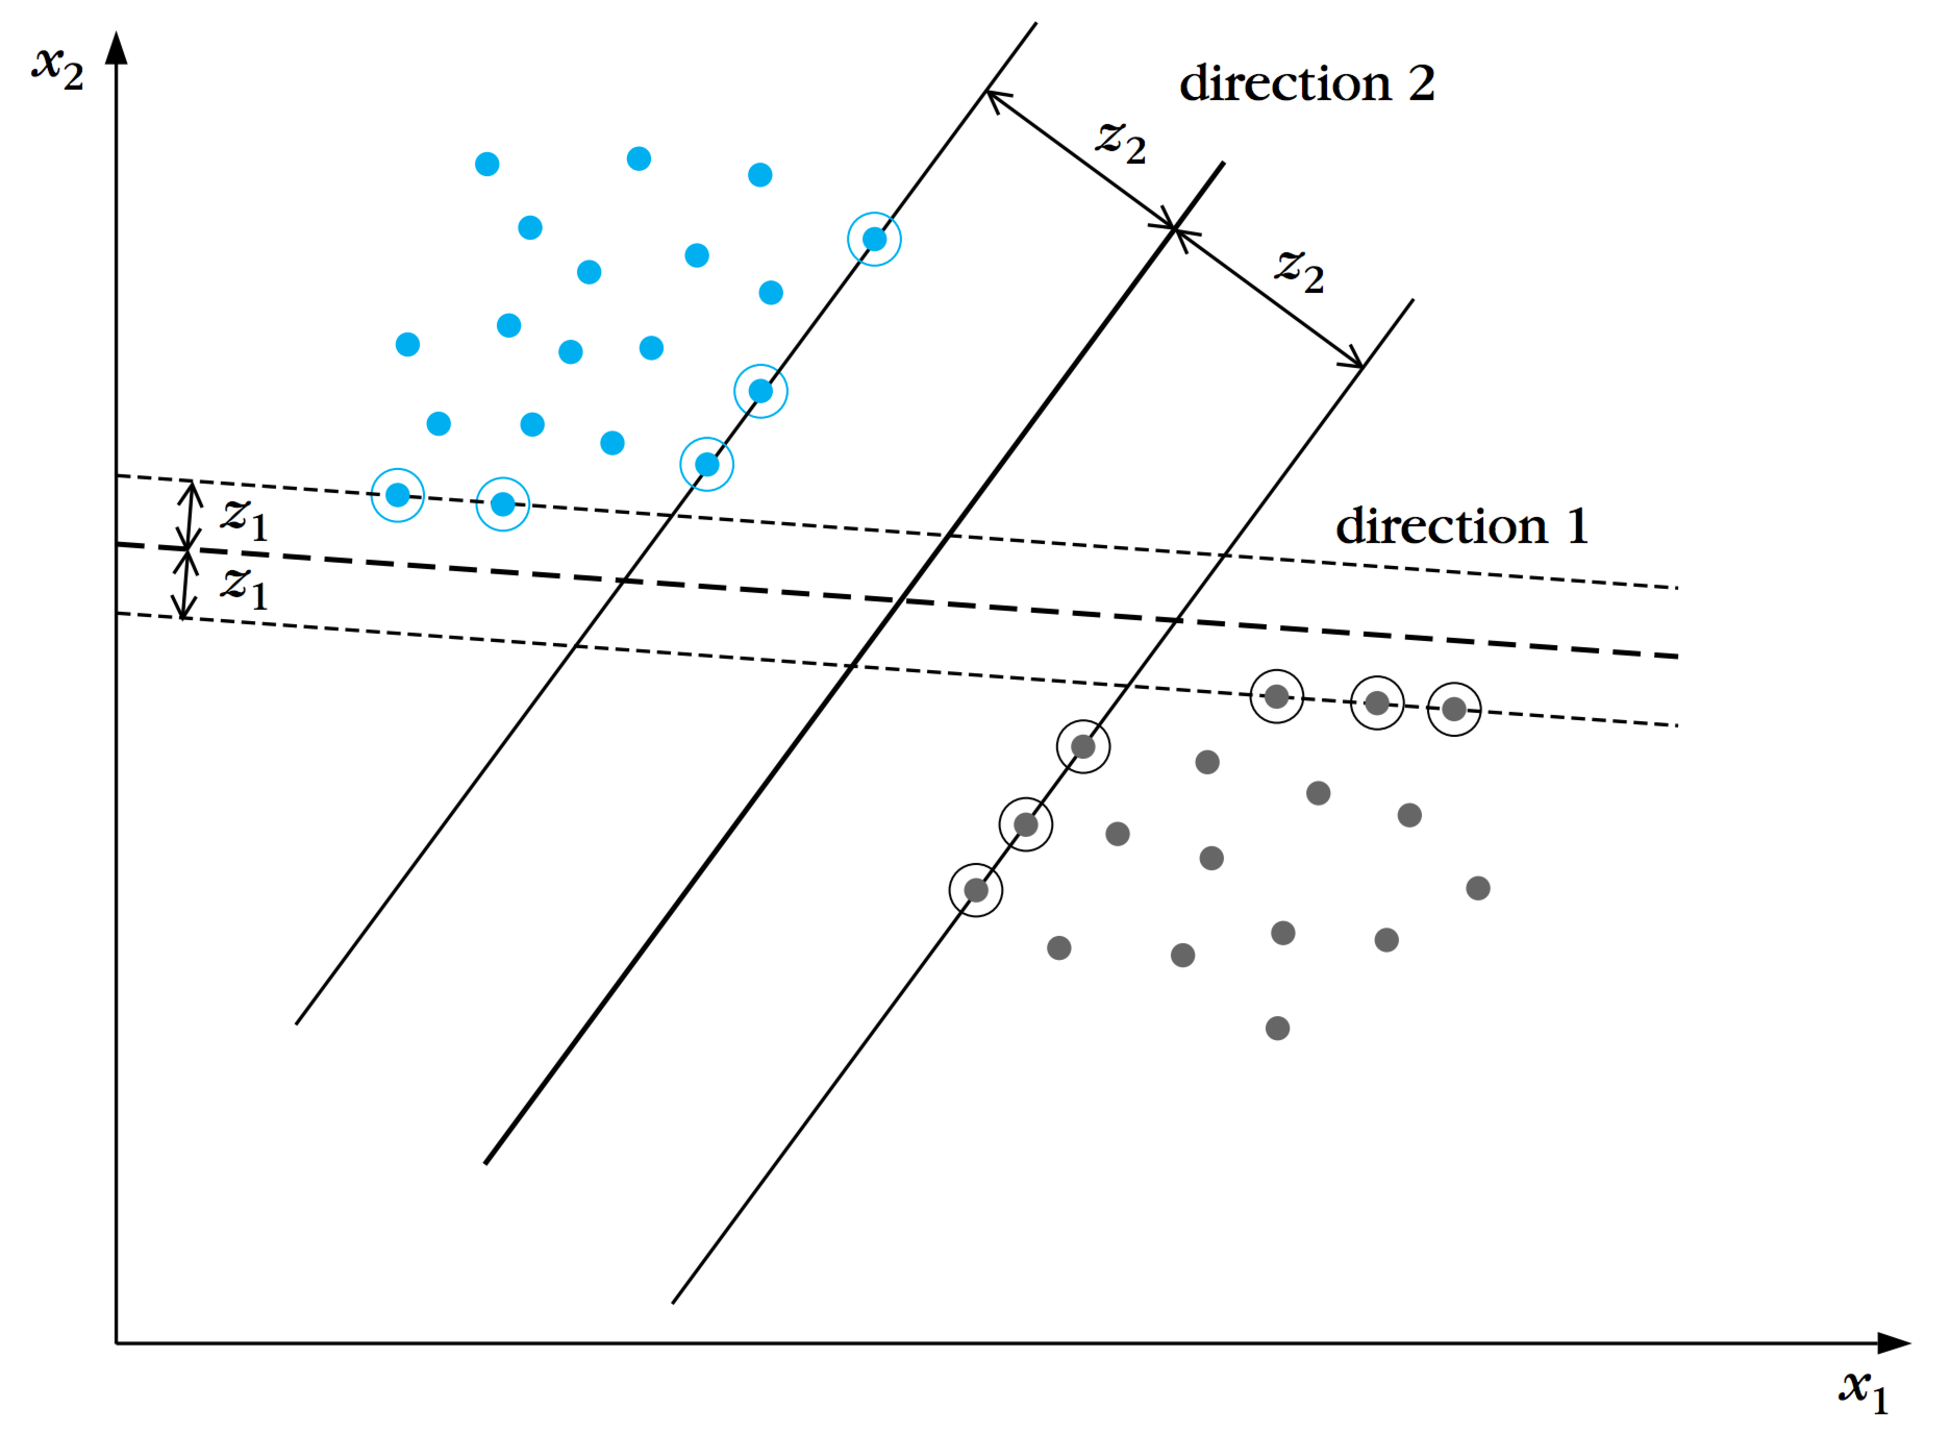
\includegraphics[width=0.48\textwidth]{images/support-vector-machine-linear.pdf}
\caption{An example of a linearly separable binary classification problem with two possible linear classifiers. Support Vector Machine finds the hyperplane that maximises the marginal between the classes.~\cite{theodoridis:2009:pattern-recognition}}
\label{fig:support-vector-machine-linear}
\end{figure}

The general SVM can be extended to solve a non-separable classification problem, by allowing the inputs points to be incorrectly classified with certain cost. Further, a non-linear separation is achieved by non-linearly mapping the input features into a new feature space and using a similar SVM as in the linearly separable case. An example of the non-linear case is presented in the Figure~\ref{fig:support-vector-machine-linear-non-linear}.~\cite{theodoridis:2009:pattern-recognition}

\begin{figure}[H]
\centering
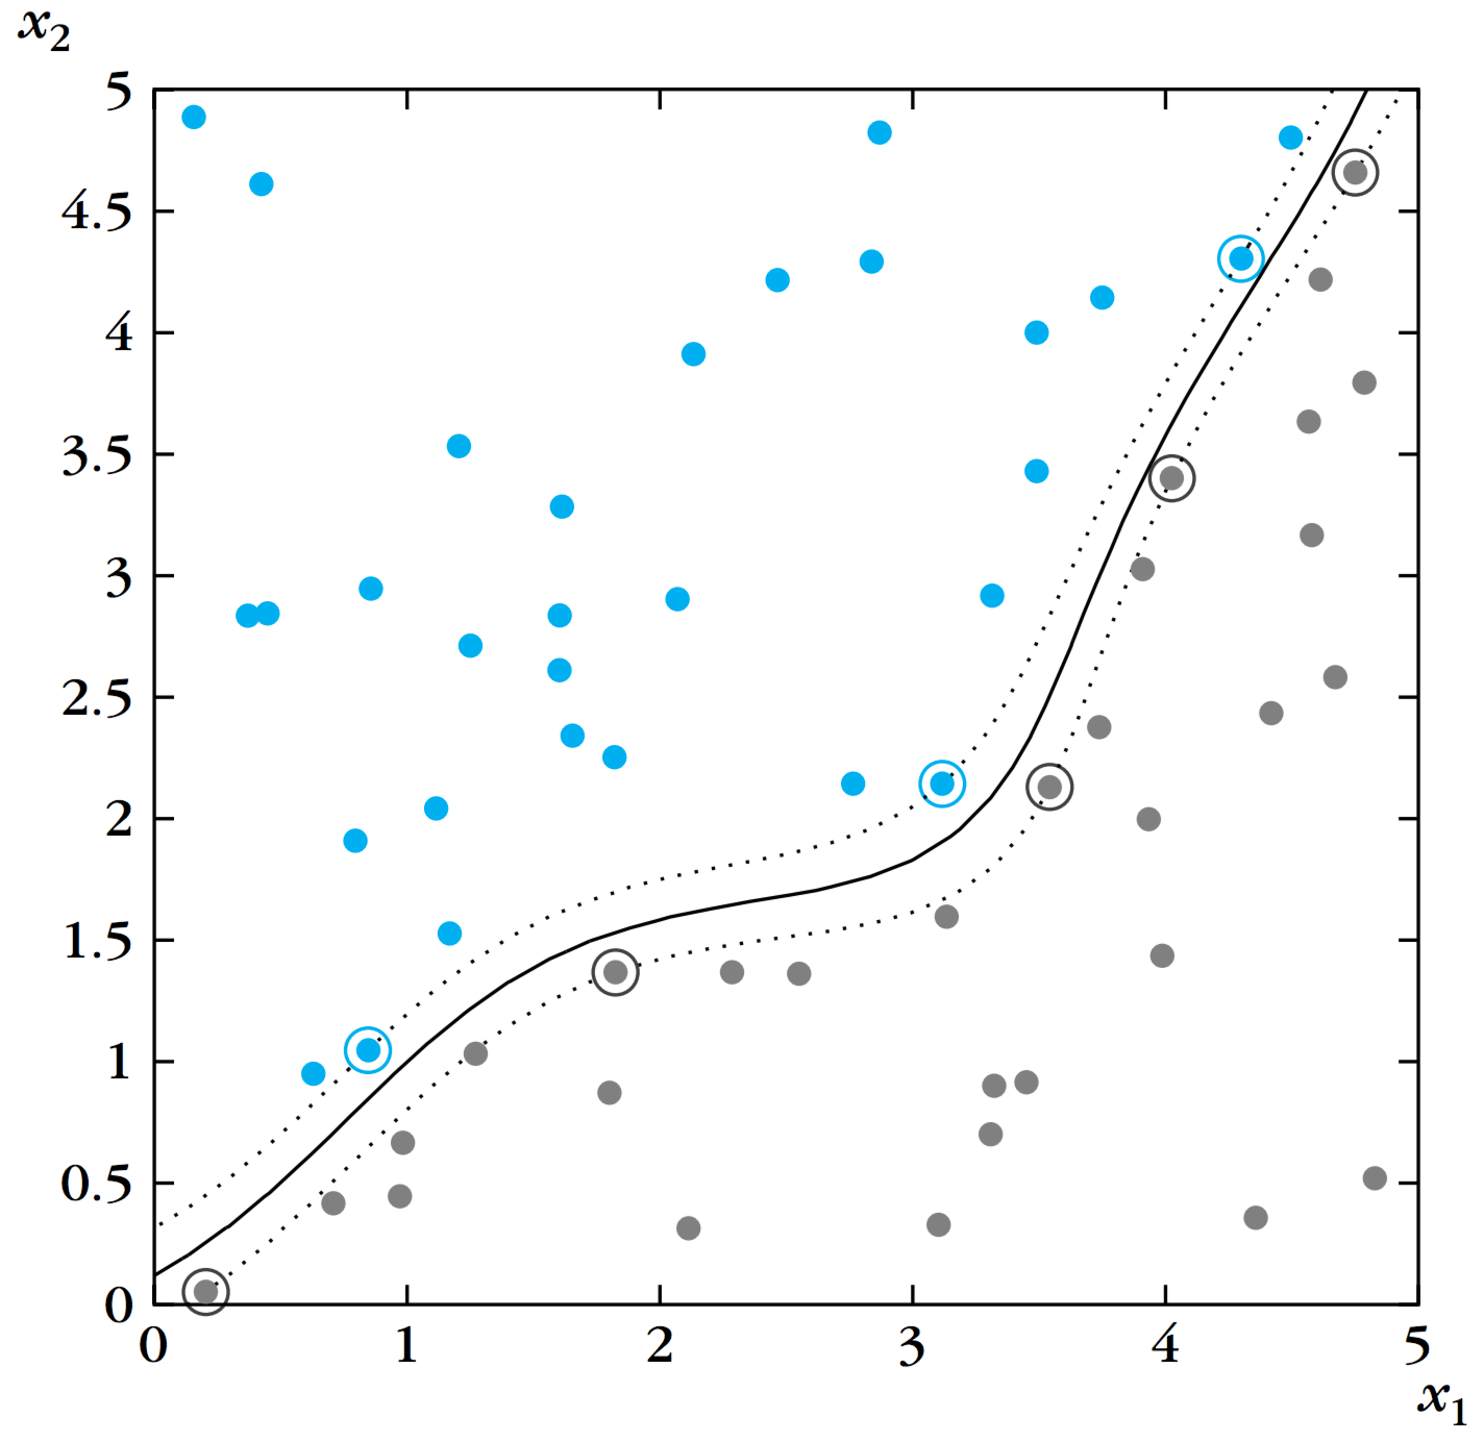
\includegraphics[width=0.48\textwidth]{images/support-vector-machine-non-linear.pdf}
\caption{An example of a classification of non-linear classification done by support vector machine.~\cite{theodoridis:2009:pattern-recognition}}
\label{fig:support-vector-machine-linear-non-linear}
\end{figure}

\subsection{Bagged Decision Trees}
One method for creating well performing learners is to combine multiple weaker learners in a way that improves the robustness of the model \cite{alpaydin:2004:introduction}. Combinations of a large number of simpler learners have performed well in machine learning competitions \cite{kaggle:2015:winner}. TreeBagger is a Matlab tool that combines decision trees using bootstrap aggregation \cite{matlab:2015:treebagger}.

The base learning algorithm used by TreeBagger is decision tree. Decision trees are a supervised nonparametric learning method. Decision trees represent the hypothesis by a tree where each leaf node corresponds to an area in the input space. The tree branches are binary decisions. The learning algorithm uses a heuristic method to select the best feature to branch by. The key idea of learning decision trees is to take advantage of the recursive property of trees that a new tree is created by attaching a tree to a leaf of another tree. \cite{alpaydin:2004:introduction}

The empirical error approximates the generalization error the better the larger the dataset is. Because the size of the real training data is limited, the training set is enlarged artificially. One way to artificially enlarge the dataset is to use the histogram of the training data as the ``true'' dataset. Using the histogram for enlarging the dataset is called bootstrap aggregation \cite{breiman:1996:bagging}. TreeBagger uses bagging to create the training datasets for the decision trees.

\subsection{Data Pre-processing}
A crucial part of successful prediction using machine learning methods is to make sure the data is in suitable form for the learning algorithm used. For example algorithms that depend on a measure of distance between the datapoints, k-NN for example, can generalize the data better when the distances are standardized. The distances are standardized by dividing the features by their standard deviations.~\cite{alpaydin:2004:introduction}.

Some learning algorithms benefit from the data being centered around zero. The centering is achieved by subtracting the mean of the data from all of the data vectors.~\cite{alpaydin:2004:introduction}

It is often beneficial to keep the models simple. It is stated that simpler models are more robust on small datasets~\cite{alpaydin:2004:introduction}. Feature selection is one way to reduce model complexity. Feature selection means selecting a subset of the data features for training the predictor. Different methods for feature selection can be used, but they are based on the same idea of repeatedly evaluating validation error on different subsets of features. The subsets can be chosen for example by starting from no features and adding the feature that improves performance the most. One way for feature selection is searching through all the combinations of features but it is often not practical due to large number of features.~\cite{alpaydin:2004:introduction}

\subsection{Model Evaluation}
To make informed decisions about how to optimize the model parameters and in general how to create good predictors, methods for comparison of the created models are needed. A simple measure of the empirical error on the training data is usually not enough. To get more accurate estimates of the generalization error, the training dataset is split into training and validation datasets. The validation dataset is not used for training of the model, as its sole purpose is to be used for estimation of the generalization error.~\cite{alpaydin:2004:introduction}

The number of labeled training samples is limited in real world machine learning problems. Therefore the size reduction to the training dataset resulting from the use of the validation set is not desirable. K-fold cross validation is a commonly used method for validation without drastic change in the training set size. In k-fold cross validation the training dataset is divided to k ``folds'' one of which is used for validation at a time and the rest for training. Each fold is used in turn for validation the generalization error estimate is the average of the errors for each of the k-folds.~\cite{alpaydin:2004:introduction}

Leave-one-out error is a variation of k-fold error where k is set to one. Leave-one-out error is often computationally prohibitively expensive.

%%% Local Variables:
%%% mode: latex
%%% TeX-master: "report"
%%% End:


%------------------------------------------------

\section{Experiments}
In the experiments two prediction tasks were studied. The first task was to classify the vinho verde dataset to red and white wines. In the second task wine qualities were approximated with regression. In this section the conducted experiments are described.

\subsection{Wine Type}
The wine type prediction was a binary classification task with two classes, namely red and white wines. Two classification methods namel k-nearest-neighbor classifier and support vector machines were studied. A k-nearest-neighbor classifier was implemented from scratch. The Matlab implementation of support vector machines was used. The experiments conducted with the two classifiers are described in the following.

\subsubsection{K-Nearest-Neighbor Classifier}
A K-Nearest-Neighbor classifier was implemented. The implementation details are given in appendix~\ref{appendix-a}. In the model selection phase different parameters were experimented with and the results were validated using 20-fold cross validation. The only preprocessing step for the data was centering, meaning making the data zero mean and unit variance.

The parameter space for a model as simple as kNN classifier is large. To limit the required work and computation time, only the most influential parameters were experimented with. The number of neighbors $k$ was the most influential parameter. Values of $k$ from 1 to 50 were tested. Another parameter that was experimented with was the distance function. Euclidean distance and Minkowski distance were tested.

\subsubsection{Support Vector Machine}
Support Vector Machines were studied for the classification task. Matlab has a versatile SVM implementation included in the default distribution~\cite{matlab:2015:fitcsvm}. The Matlab SVM implementation has a multitude of parameters to tune and the total parameter space is huge. To help reduce the number of parameters to be tested, the Matlab classification toolbox was used to find coarse parameters.

Three different kernel functions were used. Quadratic and cubic kernel functions performed poorly compared to the gaussian kernel functions and they were excluded from further experiments. The gaussian kernel functions were studied using by setting the box constraint to 1 and testing the kernel scale $\gamma$ with values in the range 0.1-20.

20-fold cross validation was used for the model selection.

\subsection{Wine Quality}
\subsubsection{Multivariate Linear Regression}
10-fold cross validation

\subsubsection{Bootstrap Aggregation with Decision Trees}
validation: OOBPrediction
\subsubsection{Extreme Learning Machine}
neuronit: 11 linear neurons, for linear riippuvuus
nonlinearty: tansig 0 - 1000
leave-one-out validation



% \begin{table}[H]
% \caption{My current knowledge of tables}
% \centering
% \begin{tabular}{cc}
% \textbf{Table type} & \textbf{Likely location}\\
% \midrule
% Coffee table & Living room\\
% Dining table & Dining room\\
% Bedside table & Bedroom
% \end{tabular}
% \end{table}

%%% Local Variables:
%%% mode: latex
%%% TeX-master: "report"
%%% End:


%------------------------------------------------

\section{Results}
The results for the wine type and wine quality predictions are presented in the Tables \ref{tab:type-results} and \ref{tab:quality-results}, respectively.

\begin{table}[H]
  \caption{Results for the wine type predictions}
  \centering
  \begin{tabular*}{0.48\textwidth}{c|c|c}
    \textbf{Method} & \textbf{Parameters} & \textbf{Accuracy [\%]} \\
    \midrule
    k-NN & Euclidean, k=6 & 94.0 \\
    SVM  & Gaussian, $\gamma=2.85$ & 99.125 \\
  \end{tabular*}
  \label{tab:type-results}
\end{table}

\begin{table}[H]
  \caption{Results for the wine quality predictions}
  \centering
  \begin{tabular*}{0.48\textwidth}{c|c|c}
    \textbf{Method} & \textbf{Parameters} & \textbf{Accuracy [\%]} \\
    \midrule
    Linear Regression & - & 49.75 \\
    ELM & l=11, nl=1 & 54.75 \\
    Bagged Trees & 250 trees & 68.25 \\
  \end{tabular*}
  \label{tab:quality-results}
\end{table}


For the wine type prediction task, the k-Nearest Neighbor classifier achieved 94.0\% accuracy, using euclidean distance and 6 nearest neighbors. The best prediction accuracy for Support Vector Machine, 99.125\%, was achieved using Guassian kernel function with the kernel parameter $\gamma=2.85$.

For the wine quality prediction task, the Bagged Decision Trees outperformed the Extreme Learning MAchine and the linear regression model. The final extreme learning machine consisted of 11 linear neurons, and 1 non-linear neurons, achieving 54.75\% accuracy. The linear regression, with no specific hyperparameters, achieved 49.75\% accuracy, and the Bagged Decision Trees, using 250 trees, achieved 68.25\% accuracy.


% ELM: 11 linear, 1 non-linear, accuracy: 0.54750
% linear regression: accuracy: 0.49750
% TreeBagger: 68.25, 250 trees

% kNN: k=6, accuracy = 94.0
% SVM: kernel scale 2.85, gaussian kernel, accuracy = 0.99125

%%% Local Variables:
%%% mode: latex
%%% TeX-master: "report"
%%% End:


%------------------------------------------------

\section{Discussion}
\label{sec:discussion}

%%% Local Variables:
%%% mode: latex
%%% TeX-master: "report"
%%% End:


%----------------------------------------------------------------------------------------
%	REFERENCE LIST
%----------------------------------------------------------------------------------------

\bibliographystyle{plain}
\bibliography{references}{}

%------------------------------------------------

\section*{Appendix A}
\label{appendix-a}
%%% Local Variables:
%%% mode: latex
%%% TeX-master: "report"
%%% End:


%----------------------------------------------------------------------------------------

\end{multicols}

\end{document}

%%% Local Variables:
%%% mode: latex
%%% TeX-master: t
%%% End:
